%!TEX root = ../main.tex

\subsection{Go-Kart CAN protocol (GoCAN)}\label{sub:CAN_protocol}
Due to the requirements of the on-kart network, it was decided to formulate a new protocol specifically for this project.
While CANopen could be used, it is a vast protocol with many features that are of no use in this system.
An elaboration of the choice to make a custom protocol over using CANopen is done in this section.
Additionally, the design of the go-kart CAN protocol, or GoCAN for short, is also presented.
The requirements of GoCAN are listed below.

\begin{itemize}
	\item Simple and easy to learn.
	\item Support for 16 nodes.
	\item One node must be able to receive/transmit data to/from multiple inputs/outputs
	\item Publish/subscribe architecture.
	\item Variable data length - beyond 8 bytes per message
	\item Expandable -- must be able to add more nodes without affecting the existing ones.
	\item Commands: Start/stop broadcasting 
	\item Commands can be send to specific or all nodes
	\item Timestamp data
\end{itemize}

\thomas{This is changed!}
\subsubsection*{The CANopen Protocol}
\label{sub:CANopen}
As mentioned before, CANopen is a high level protocol that runs on top of the CAN protocol.
It is open source project, that runs on the top 5 layers of the OSI model\cite{CANopen_introduction}.
It includes several types of protocols, most interesting are the SDO and PDO. 
By splitting the 11 bit Message ID into a 4 bit function code, followed by 7 bits of node ID, meaning that a node can communicate 16 different functions to 127 different nodes.
\\~\\
The Service Data Object (SDO) can read from or write to any registers on any node. 
It can handle 127 different nodes with each 65536 different indices, each with 256 sub indices, in total, more than 2 billion addresses with each 4 bytes of data.
The way CANopen supports this, is by using the first four bytes of the data portion of the frame for metadata, as described in figure~\ref{fig:CANopen_SDO_data}.
This of course means that the overhead from one message increases from 47 bits to 79 bits, or 247 \% of the maximum data size.\\

\begin{figure}[h]
	\centering
	\includegraphics[width=0.9\linewidth]{graphics/CANopen_SDO_data_crop}
	\caption{"The data section of the CAN frame is split into three parts: one byte for the specifier, three bytes for the node index and subindex, and four bytes for the actual data in the transfer."\cite{CANopen_introduction}}
	\label{fig:CANopen_SDO_data}
\end{figure}

\todo[inline]{I clarefied some of the calculations. }
This protocol is not ideal for this network. 
In part because it's request based, but more because of the enormous overhead.
For instance, the IMU produces 4 byte data types for each of its 9 axes. 
With an overhead of 79 bits, this comes to 999 bits, and at 400 Hz, that node alone will take up 40 \% of the bandwidth.
In addition to this, all transmits would need to be requested, so the total bandwidth comes close to 70 \%.
%Metadata is 47 bits, plus 32 bits from the Data portion. The data it self is a float, so that's 32 bits; 111 in all. A request does not include data, so that's only 79 bits of data. At 400 Hz, that's (111+79)*9*400=684000.
The SDO is generally used to define or read parameters for that node, that are not bound to change over time.
It should not be used for broadcasting data.
\\
The Process Data Object (PDO) is a protocol used to transmit specific indices with a higher throughput. 
In this protocol, certain indices are mapped to one of 8 PDOs per node. 
This way, a node can identify data only by the CAN message ID, without using any of the data portion for overhead.
It is also possible to group multiple values together, and to transmit without request, either at fixed time or event driven.
Using PDO, it is possible to group 8 of the axes together and send the 9th by itself.
This brings the data from the IMU down to 523 bits to transmit its 9 axis data.\\
%((32+32)+47)*4+(47+32)

Each node on the CANopen bus has its own Object Dictionary (OD) specifying its addresses. 
Some of these addresses are reserved, but since the Message ID specifies which node it is, there's no risk of overlapping.
If then one part is replaced by a different make or model, then it might be necessary to reconfigure other nodes, and the system loses modularity.\\

For all its nice features, the CANopen protocols do not fit the requirements outlined in the beginning of this section. 
It includes a lot of complexity, which unnecessary for this project.
Instead it has been decided to develop a custom High Level Protocol that relies more on the automatic functionality of the CAN protocol.\\

\subsubsection*{The GoCAN Protocol}
The basic CAN frame is retained for this protocol.
GoCAN, mostly, is a reinterpretation of the message ID of the frame.

\begin{figure}[h!]
	\centering
	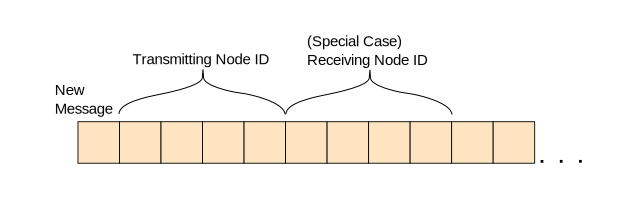
\includegraphics[width = 0.9\linewidth]{graphics/CAN_protocol_general}
	\caption{Naming convention for this high level protocol}
	\label{fig:CAN_protocol_general_pdf}
\end{figure}
\thomas{Indicate messageid, remove color in dotted box, split into two cases}
The message ID is split into three portions, as seen on figure~\ref{fig:CAN_protocol_general_pdf}.
The first bit is set to 1 if this is a new message.
If the node needs to send more than 8 bytes in one message, this bit can be set to 0, thus blocking other nodes with higher priority.
The subsequent four bits indicate the transmitting node ID, which will allow up to 16 nodes. 
The last 6 bits of the message ID determine the message type. 
This leaves 64 different message types for each node.
It is the responsibility of the developer to utilize these correctly.\\

There are two types of nodes: 
\begin{itemize}
	\item \textbf{The Wifi node:} Acts as the link between the user on the monitoring station and the network.
	It transfers data to the monitoring station and distributes commands on the network.
	\item \textbf{Sensor nodes:} Any sensor or data producing unit will be associated with a node.
	A sensor node will produce data and act according to received commands
\end{itemize}


In this case, the subsequent four bits determines the recipient, leaving two bits for command type. 
For now, command types are "Start broadcasting", "Stop broadcasting" and "Synchronize".
These will be explained in more detail in section \ref{sec:CAN_functions}.
If the recipient message ID is the WiFi node ID, then the command applies to all nodes.\\
\thomas{Reference to figure msg id}

The four node IDs currently in use:
\begin{table}[h]
	\begin{tabular}{{l} {l}}
		Wifi node: & 0b0001 \\
		IMU node: & 0b0011 \\
		Sevcon node: & 0b0111 \\
		GPS node: & 0b1110
	\end{tabular}
\end{table}

The WiFi node is given the lowest node ID since this will result in the highest priority.
This is necessary when issuing commands.
The IMU produces short data packages at a high rate, and the GPS node produces data packages at a lower rate. 
Therefore it is of less concern if the GPS message is delayed due to obstruction from other nodes. 
